\chapter{Pruebas de performance sobre el caso de estudio}
\label{capitulo7}
\section{Introducción}

De acuerdo con las buenas prácticas recopiladas de la bibliografía consultada y detalladas en la sección \ref{capitulo3:reglas} las modificaciones realizadas sobre Diaspora deberían 
redundar en mejoras en la performance de la misma. Para evaluar las mejoras se desarrolló un conjunto de pruebas de performance, siguiendo las ideas presentadas en el 
Capítulo \ref{capitulo2}. En este Capítulo se presentan las pruebas desarrolladas. En la Sección \ref{cap7:ambiente} se describe la preparación del ambiente de pruebas. Luego, en la 
Sección \ref{cap7:herramientas} se presentan las herramientas utilizadas, en la Sección \ref{cap7:prep_pruebas} se presenta la preparación de las pruebas. Finalmente en la Sección 
\ref{cap7:plan} se presenta el plan de pruebas, y por último en la Sección \ref{cap7:resultados} se muestran los resultados obtenidos y un análisis de los mismos.

\section{Ambiente}
\label{cap7:ambiente}

Para realizar las pruebas fue necesario configurar un ambiente que fuera lo más parecido a la configuración de producción de \emph{Diaspora}. El equipo consta de 
un procesador pentium IV, 2 GB de RAM, corriendo la versión 12.04 de Ubuntu server. El ancho de banda del que se dispuso fue de 120 Mb de poder de 
descarga y 10 Mb de poder de subida..

Como manejador de base de datos se utilizó \emph{Postgres}. Otra vez, la decisión estuvo basada en la tendencia de la industria. Hasta hace algunos años, la mayoría de las
aplicaciones construidas con \emph{Ruby on Rails} utilizaban \emph{Mysql}. La corriente empezó a cambiar cuando \emph{Mysql} fue
adquirido por \emph{Oracle} y la performance y funcionalidades de \emph{Postgres} mejoraron \cite{nginx_vs_apache}. La versión utilizada de \emph{Postgres} es la 9.1.5.

Para poder realizar liberaciones de distintas versiones de código, existe un mecanismo amigable para aplicaciones \emph{Ruby on Rails}. El paquete \emph{capistrano} \cite{capistrano} es el  utilizado 
en la actualidad por la mayoría de las aplicaciones construidas con \emph{Rails}. El funcionamiento es bastante transparente para el desarrollador, el paquete se debe incluir en el 
\emph{Gemfile} y realizar algunas configuraciones. Una vez configurado correctamente, cualquier persona con los permisos correspondientes puede realizar
liberaciones al ambiente remoto deseado con un solo comando desde la consola.

Para la elección del servidor web se tuvieron en cuenta las siguientes opciones, \emph{Apache} \cite{apache} y \emph{nginx} \cite{nginx}. Se optó por utilizar \emph{nginx} debido a que la tendencia en los 
últimos años en la industria ha virado hacia el mismo como se puede ver \cite{nginx_vs_apache}. Esto se debe a que se trata de un servidor más ligero, que consume menos memoria 
en pedidos concurrentes debido a la definición de su arquitectura. \emph{Apache} maneja los pedidos con una arquitectura basada en la creación de hilos en procesos que puede 
volverse pesada al tener que manejar muchos usuarios concurrentes. En cambio \emph{nginx} está basado en una arquitectura basada en eventos, la cual consume menos recursos 
en promedio \cite{nginx_perf}. Se utilizó la última versión estable, la 1.2.3.

Como servidor de aplicación se utilizó \emph{Thin} \cite{thin}. En este caso se disponía de dos alternativas principales, el mencionado y \emph{passenger-phusion} \cite{phusion_passenger}. Éste último, era
el estándar cuando se utilizaba \emph{Apache} como servidor web, pero con el cambio a \emph{nginx} el estándar se volvió \emph{Thin}. La versión utilizada de \emph{Thin} es la
1.4.1.

Para el control de versiones se utilizó \emph{Git} \cite{git}, debido a que utiliza un sistema de ramas liviano el cual permite dividir el estado del proyecto de manera ágil, esto permite
tener varias ramas con distintas mejoras por separado, y cambiar entre ellas de manera fácil para realizar pruebas.

\section{Herramientas utilizadas}
\label{cap7:herramientas}
\subsection{\emph{JMeter} y \emph{New Relic}}

Imitar las interacciones que realiza un usuario con un sitio es muy difícil de recrear, y lo es aún más en cantidades que generen mediciones relevantes para performance.
Además existen otros problemas, siendo el problema principal que estas herramientas simulan los pedidos realizados por un navegador web y no su comportamiento \cite{jmeter}.

En el navegador cuando se accede a un sitio, se realiza un pedido inicial cuya respuesta contiene el documento HTML que se desplegará. Una vez descargado el documento principal, 
existen otros pedidos que el navegador debe realizar para obtener el resto de los recursos que hacen que el sitio termine de cargar su comportamiento. En este período de carga 
existen ciertas restricciones que los navegadores aplican al realizar los pedidos subsiguientes \cite{souders2007high}. Por ejemplo, cuando se realiza un pedido de un recurso de tipo 
\emph{javascript}, el resto de los pedidos se paralizan. Esto se debe a que luego de descargar un \emph{script}, el navegador debe analizarlo, y ejecutarlo, y este potencialmente 
puede cambiar la estructura del \emph{DOM}.

\emph{JMeter} no se comporta de la misma manera que un navegador, por lo cual la simulación se ve afectada. En la realidad de \emph{Diaspora} esto es particularmente importante, 
ya que muchas de sus funcionalidades utilizan \emph{backbone} que se ejecuta totalmente del lado cliente. La única funcionalidad que provee \emph{JMeter} es analizar 
sintácticamente el HTML devuelto por el servidor, buscar enlaces dentro del mismo, y realizar los pedidos a las \emph{URLs} correspondientes. Otro problema en la simulación del
comportamiento del navegador, es que éste varía dependiendo del navegador utilizado, teniendo cada uno de ellos heurísticas distintas para resolver distintos problemas. Así que por 
más que \emph{JMeter} sea una buena herramienta para simular muchos usuarios simultáneos, sus resultados están sesgados por sus capacidades, en especial por la falta de 
ejecución del código en el lado cliente. De todas formas, se utilizó \emph{JMeter} para pruebas con carga alta de usuarios y para simular un sitio con alto uso al realizar las pruebas 
del lado cliente.

\emph{New Relic} es una herramienta de diagnóstico que brinda estado sobre el servidor al que se lo aplique en tiempo real. En el caso del proyecto, fue configurado para
obtener estadísticas del servidor de pruebas, como por ejemplo, recursos físicos y ancho de banda consumido. \emph{New relic} también brinda la posibilidad de obtener
detalles de la aplicación, como por ejemplo, páginas visitas, el \emph{throughput} y el tiempo medio de respuesta.

\subsection{\emph{Page Speed}, \emph{YSlow} y \emph{WebTestPage} }

Estas herramientas se utilizaron para tomar métricas fieles a las características de los navegadores, que como se especificó en la sección \ref{cap7:herramientas}, es muy difícil con
herramientas de generación de carga como \emph{JMeter}. Además, estas herramientas realizan sugerencias que van alineadas a las reglas de performance del lado cliente, descritas 
anteriormente. Es por esto que se utilizaron para validar mejoras del lado cliente realizadas en \emph{Diaspora}. 

\section{Preparación de las pruebas}
\label{cap7:prep_pruebas}
\subsection{Datos de Prueba}

Los datos de prueba de mejor calidad, serían utilizando una copia de la base de datos de \emph{Diaspora} en producción. Se pidió un \emph{dump} de la base de datos de
producción a uno de las encargados de mantenimiento de \emph{Diaspora}. El pedido fue denegado debido a que en los datos se encuentra información sensible de los
usuarios. En vista de esto, se procedió a pedir datos estadísticos de las actividades de los usuarios en producción. A partir de éstos, se trató de 
generar un conjunto de datos de prueba mediante un \emph{script} que reprodujera la estadística.

De todas formas, reproducir los datos con un \emph{script} es propenso a generar errores de consistencia en la base de datos. Esto se debe a que cuando el usuario realiza
acciones en el sitio, cada acción desencadena potencialmente varios cambios en la base dependiendo del usuario en ese momento, y de los parámetros que envió desde
el lado cliente del sitio. Esto implica que realizar un \emph{script} que contemple realidades complejas sea difícil de construir y validar.

Aplicando los criterios presentados en la Sección \ref{cap2:modelado_uso} sobre como modelar la realidad, y las estadísticas provistas por \emph{Diaspora}, se creó un conjunto de 
datos de pruebas. En la figura \ref{fig.datos_de_prueba}, se representan los cuatro conjuntos de usuarios creados, donde cada una de ellos tiene a todos sus miembros 
conectados entre sí. Además, todos los miembros de cada grupo siguen \emph{tags} del mismo tipo, simulando un interés común. En cada conjunto existen 
algunos miembros que también están conectados con miembros de otros conjuntos. La idea es simular grupos grandes de usuarios conectados entre sí por un porcentaje 
relativamente pequeño de usuarios. 

\begin{figure}[h!]
\centering
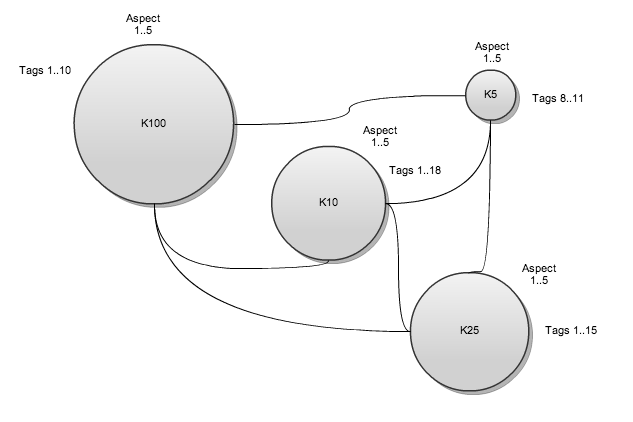
\includegraphics[scale=0.5]{figuras/figura_datos_prueba.png}
  \caption{Estructura de los datos de pruebas generados}
    \label{fig.datos_de_prueba}
\end{figure}

Una vez creada esta estructura se generó un archivo de respaldo realizado con el programa \emph{pg\_dump} para poder restablecer el estado de la base de datos en caso
de que las pruebas la modificaran y agilizar así el proceso de pruebas.

\section{Plan de pruebas}
\label{cap7:plan}

Los casos de uso más utilizados se determinaron a partir de conversaciones con los encargados de mantenimiento de \emph{Diaspora}. A continuación se listan los casos de
pruebas creados por el equipo para representar los casos de uso más comunes.

\subsection{Casos de prueba}

\subsubsection{Caso de prueba 1: visita a \emph{stream}}

Esta prueba consta de simular el caso de uso conformado por el inicio de sesión de un usuario, y la visita a su \emph{stream}. Este caso de uso es el principal y más básico, ya que 
todos los usuarios que utilizan \emph{Diaspora} deben seguir este flujo.

\subsubsection{Caso de prueba 2: visita a \emph{aspects}}

Esta prueba reutiliza el caso de prueba 1, y complementa al mismo con otra funcionalidad muy utilizada que es la de visualizar los distintos \emph{aspects} o grupos de contactos
de los usuarios. El caso comprende el inicio de sesión, la visita a su \emph{stream}, y la visita a cada uno de los \emph{aspects} del mismo, esto genera que el
contenido del sitio varíe según el grupo de contactos que el usuario haya seleccionado.

\subsubsection{Caso de prueba 3: visita a \emph{tags}}

Esta prueba reutiliza el caso de prueba 1, y luego simula el acceso por parte de un usuario a todas las \emph{tags} que se generaron en los casos de pruebas. Visitar una
\emph{tag} genera contenido variable dependiendo del usuario, sus contactos, y del nivel de privacidad de las publicaciones. Al iterar sobre todas las \emph{tags} de la
aplicación con distintos usuarios se producen consultas y resultados variados en el servidor.

\subsubsection{Caso de prueba 4: visita a \emph{contacts}}

Esta prueba también reutiliza el caso de prueba 1, y además accede a la página \emph{contacts} del usuario, listando todos los contactos que el usuario tiene asociados
en el sitio.

\subsubsection{Caso de prueba 5: visita a perfiles de contactos}

Esta prueba vuelve a utilizar el caso de prueba 1, y accede a perfiles de distintos usuarios, uno de los casos más comunes de la realidad. Este caso intenta representar
el acceso de un usuario al perfil de sus contactos a través de alguna publicación de interés, o la búsqueda de nuevos contactos, accediendo a perfiles de usuarios desconocidos.

\subsection{Detalles de la implementación de las pruebas}

Dado que muchas de las funcionalidades más usadas de \emph{Diaspora} están construidas en \emph{backbone}, muchos de los pedidos que se realizan al servidor son a través
de la interfaz \emph{javascript} provista por la herramienta. Como \emph{JMeter} no es capaz de analizar y ejecutar \emph{javascript}, además de no ser capaz de simular los 
eventos producidos por un usuario (por ejemplo: hacer \emph{click} en un botón), existen ciertas limitantes que se recrearon de la forma que se creyó mejor.

\emph{JMeter} permite analizar la respuesta a un pedido HTTP por un documento HTML y generar sub pedidos para obtener los recursos que son referenciados por una URL en
el documento, como imágenes, hojas de estilo y \emph{javascript}. En la realidad de \emph{Diaspora}, cuando se realiza el pedido para obtener el \emph{stream} de un usuario,
el servidor retorna un documento HTML. Este documento dispara por \emph{javascript} un pedido HTTP al servidor mediante \emph{backbone} para obtener las publicaciones
de los usuarios. Luego de obtener las publicaciones en formato JSON, se modifica el documento HTML recibido mediante \emph{javascript} para desplegar las publicaciones. Al
realizar esta acción se solicitan al servidor nuevas imágenes. Para mantener las pruebas lo más fieles a la realidad posible, se usó un componente de \emph{JMeter} que permite
analizar las respuestas de los pedidos realizados por la herramienta y obtener mediante expresiones regulares las URLs de las imágenes en cuestión. Una vez obtenidas las
imágenes, se configuraron las pruebas para realizar estos pedidos, simulando lo que sucede en la realidad.

Debido a que \emph{Rails} implementa una solución al problema de \emph{cross side request forgery}
enviando un parámetro en los pedidos HTTP, llamado \emph{authenticity token}, fue necesario obtenerlo
para cada pedido mediante expresiones regulares ya que si no se encuentra dicho parámetro en el pedido
la aplicación deniega los pedidos devolviendo una respuesta de código 401 \emph{not authorized}.
 
\section{Resultados}
\label{cap7:resultados}

Para cada uno de las modificación realizadas en el código de \emph{Diaspora} detalladas en el Capítulo \ref{capitulo6} se cuenta con un directorio propio cuya estructura se ve en la
figura \ref{fig.estructura_resultados}, dentro del mismo se encuentra un archivo con extensión \emph{.jmx} para cada caso de prueba planificado. Por cada caso de prueba se 
encuentra un archivo con extensión \emph{csv} que contiene la salida generada en la corrida del caso de prueba. A partir de los datos generados en la salida de las pruebas se 
pueden analizar los resultados.

\begin{figure}[h!]
\centering
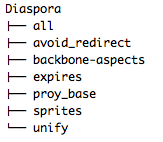
\includegraphics[scale=0.5]{figuras/est_result.png}
  \caption{Estructura de los resultados de las pruebas}
    \label{fig.estructura_resultados}
\end{figure}

Los resultados de las pruebas del lado cliente, realizadas con \emph{Page Speed} y \emph{YSlow}, se encuentran en el directorio de cada mejora, bajo el nombre
\emph{page\_speed.pdf} y \emph{yslow.pdf}.

Las pruebas fueron ejecutadas en la rama base de proyecto, en cada rama con una mejora individual, y finalmente en una que contiene todas las mejoras realizadas por el
equipo a lo largo del proyecto. Todos los resultados de las ejecuciones de las pruebas, son entregados en el anexo del informe. En esta sección se pasará a realizar un
análisis e interpretación de los resultados, comparando la rama base sin optimizaciones con la rama que contiene todas las optimizaciones.

\subsection{Resultados de pruebas del lado cliente}

El sitio oficial de \emph{Diaspora} en la página de \emph{stream}, obtiene una puntuación de sesenta y un puntos en \emph{Page Speed} y una nota de grado C en \emph{YSlow}. Es 
importante destacar que al momento de realizar estas mediciones, la versión del código en el sitio se encuentra en una versión posterior a la versión abierta al empezar el proyecto. 
Para que la comparación tenga sentido, es necesario asegurarse que las únicas diferencias entre la versión base y las versiones a comparar, sean las mejoras implementadas. Esto se 
debe a que no se desea considerar cambios realizados por personas ajenas al proyecto que impacten de alguna forma en la performance del proyecto, afectando la validez de los 
resultados.

En el ambiente de pruebas recreado por el equipo, con la versión base del código, el sitio obtiene una puntuación de cincuenta y seis puntos en \emph{Page Speed} y una nota de
grado C en \emph{YSlow}. Como se puede ver, existen diferencias de puntaje que se pueden deber a los siguientes factores:

\begin{itemize}
	\item
	Cambios en el código, algunas de las mejoras del equipo ya se encuentran en el sitio en producción actualmente.
	\item
	El sitio en producción utiliza CDNs para distribución de recursos y para guardar imágenes subidas por los usuarios, por lo que estas herramientas brindan más puntos.
	\item
	El contenido de las páginas difiere, habiendo diferentes imágenes en algunos sitios externos a \emph{Diaspora} que no se encuentran optimizadas, y que las herramientas
	no son capaces de diferenciar.
\end{itemize}

Sin embargo, la mayoría de las mejoras sugeridas por las herramientas al ambiente de pruebas, se corresponden a sugerencias al ambiente de producción. A continuación se muestra 
una lista de las mejoras más necesarias según \emph{Page Speed}
\begin{itemize}
	\item
	Combinar imágenes en \emph{CSS Sprites}.
	\item
	Habilitar compresión de recursos de tipo hojas de estilo y \emph{javascript}.
	\item
	Habilitar \emph{caching} en recursos que lo ameriten.	
\end{itemize}

Utilizando las herramientas sobre el ambiente de pruebas con la aplicación con todas las mejoras incluidas, \emph{Page Speed} le otorga noventa y dos puntos, y \emph{Yslow} le 
asigna una nota de grado A. Otro detalle a considerar es que ninguna de las herramientas realiza ninguna sugerencia crítica. Esto quiere decir que las mejoras sugeridas por las 
herramientas luego de los cambios introducidos por el equipo, serían de muy poco impacto. Luego de los cambios realizados por el equipo, el puntaje del sitio se encuentra dentro 
del rango de los puntajes de los diez sitios más visitados.

\subsection{Impacto en los casos de uso más utilizados}

Para evaluar las mejoras obtenidas por las optimizaciones implementadas, se ejecutaron los casos de uso implementados en \emph{JMeter} especificados anteriormente. Cada
ejecución fue configurada para lanzarse con diez hilos de ejecución en paralelo. Se define \emph{tiempo promedio del caso de uso}, como el tiempo promedio que le lleva a un 
usuario simulado completar el caso de prueba. 

\subsubsection{Caso de Prueba 1}

Para el caso de prueba 1, con la versión del código sin optimizaciones, simulando cincuenta usuarios por hilo, la cantidad total de pedidos realizados a la aplicación fue de
25.000. De estos pedidos, 2.500 fueron por recursos de tipo \emph{javascript}, 3000 fueron por recursos de tipo hojas de estilo, y 14.500
por recursos de tipo imagen. Discriminando los resultados por el código de respuesta HTTP, se puede que ver que el servidor respondió con código 304 1660
veces. El servidor redirige al usuario con código 301 y 302 en 1.500 oportunidades.

El tiempo promedio del caso de uso sin las optimizaciones fue de 18.8 segundos, este número está conformado por el tiempo promedio de respuesta para los 
pedidos del caso de uso. Es importante tener en cuenta que este número no representa la realidad exactamente, ya que como se detalló en otras secciones, el comportamiento del 
navegador difiere del comportamiento de \emph{JMeter}. Sin embargo, es posible comparar este número con el número generado al ejecutar el caso de prueba con las 
optimizaciones. Además una mejora en este número representaría de todas maneras una mejora en la realidad, ya que al mejorar el tiempo promedio de respuesta de cada pedido, se 
reduciría el tiempo total necesario. La cantidad promedio de \emph{KB} recibidos por usuario  fue de 481.

Con el código que incluye todos las optimizaciones, la cantidad de pedidos realizados por la ejecución de la prueba fue de 17.679. De estos
pedidos, 500 son por recursos de tipo \emph{javascript}, 3.000 corresponden a hojas de estilo y 9.679 a imágenes. Con las mejoras realizadas, el 
servidor no responde nunca con código 304 para este caso de prueba. En esta oportunidad el servidor redirigió al usuario 1.000 veces. El tiempo promedio de respuesta con las 
modificaciones fue de 21 segundos. La cantidad promedio de \emph{KB} recibidos por usuario luego de fue aplicar todas las mejoras fue de 514.

La cantidad de pedidos total se redujo en un 29\%. En caso de los recursos \emph{javascript}, la cantidad de pedidos se redujo en un 80\%, explicado por la unificación realizada. 
Cada usuario realiza un pedido por todo el \emph{javascript} de la aplicación cuando antes realizaba cinco. La ausencia de respuestas con código 304 se explica por el 
\emph{caching} de las imágenes implementado.

La reducción en la cantidad de pedidos por recursos de tipo imagen fue de 33\%. La reducción se debe en parte al \emph{caching}, pero también se debe a la implementación del 
\emph{CSS sprite}. Con el mismo, cada usuario realiza diez pedidos menos en su flujo, lo cual implica que  se realicen 500 pedidos menos.

El tiempo promedio de duración del caso de uso por usuario se redujo en un 12\%. La reducción de las redirecciones se debe a la mejora implementada en el caso de inicio de
sesión detallada en la sección de mejoras sobre \emph{Diaspora}.

Analizando la cantidad de \emph{KB} transferidos, se puede ver un incremento del 7\%. Este incremento se debe a que la imagen que se utiliza en la implementación de los
\emph{CSS Sprites} está compuesta por un conjunto de imágenes mayor a las que se pedían individualmente sin la mejora. Esto parecería ser un deterioro en la performance, sin
embargo como se detalló en \ref{cap3:reglas:menos_pedidos}, reducir la cantidad de RTT es la manera más efectiva de mejorar la performance y aprovechar el ancho de banda.
Además el \emph{CSS sprite} implementado proporciona otra ventaja que no puede verse en este caso de prueba. Si el usuario siguiera utilizando otras funcionalidades de la
aplicación, donde se necesiten estas imágenes, los pedidos no se realizarían debido a que ya estarían disponibles en el \emph{cache} del navegador. Otra de las causas del
aumento de datos transferidos durante la prueba, se debe a la unificación de recursos de tipo \emph{javascript}.

De manera similar a los \emph{CSS sprites}, todo el código \emph{javascript} de la aplicación se unificó en un archivo. Antes de la mejora, solo se realizaban pedidos por los archivos 
necesarios, los cuales en suma implicaban mucho menos tamaño que todo el código combinado en uno. Como en el caso de los \emph{Sprites} esta mejora apunta a reducir la 
cantidad de RTTs, además de que cuando el usuario utilice más funcionalidades, el código necesario del lado cliente ya va a estar disponible desde el \emph{cache} del navegador.
Además de los archivos \emph{javascript} de la aplicación, también se incluyen dentro del archivo unificado, todas las librerías externas como \emph{jQuery} cuyo tamaño en
\emph{KB} es bastante elevado. Una solución a este problema podría ser excluir la librería del archivo unificado y utilizar una CDN para el mismo los cual proporciona varias
ventajas. Como las librerías se utilizan en varias aplicaciones, al utilizar una CDN existen la posibilidad de que el navegador del usuario ya contenga una versión de las mismas en su 
\emph{cache}. Sin embargo en el caso de \emph{Diaspora}, algunas librerías fueron modificadas para comprender ciertas realidades de la aplicación, porque las versiones
disponibles en el \emph{cache} del navegador no servirían.

\subsubsection{Caso de prueba 2}

Para el caso de prueba 2, con la versión del código sin optimizaciones, simulando veinte usuarios por hilo, la cantidad de pedidos realizada a la aplicación fue de 31.396 y seis.
La cantidad de pedidos a recursos de tipo \emph{javascript} fue de 1.000, de tipo hojas de estilo fue de 1.200, y de
imágenes fue de 24.393. La cantidad de respuestas del servidor con código 304 fue 13.835. Para este caso de uso, el
tiempo promedio de duración del caso de uso por usuario fue de 82 segundos. La cantidad promedio de KB por usuario recibidos desde el servidor
en este caso fue de 662.

Con las optimizaciones, se realizaron en total 14.056. La cantidad de pedidos de recursos de tipo \emph{javascript} fue de 200, de hojas
de estilo fue de 1.200, y de imágenes 9.253. El servidor no retorna ninguna respuesta con código 304. El tiempo promedio de duración
del caso de uso para cada usuario fue de un 63 segundos. La cantidad promedio de \emph{KB} recibidos por usuario fue de 640.

La reducción de pedidos totales fue de 55\%. En el caso de los pedidos por los recursos de tipo
\emph{script} la reducción fue del 80\%. En el caso de los recursos de tipo imagen la reducción fue del 62\%. Todas estas reducciones
y la ausencia de respuestas de código 304 se explican de la misma forma que en el caso de prueba uno. La reducción en el tiempo de respuesta fue de un cuarto, la cual se explica 
principalmente por la migración de los \emph{aspects} a \emph{backbone}. La reducción en el tiempo promedio del caso de uso fue de 23\% y la reducción en cantidad promedio
de \emph{KB} fue de 3\%.

Si bien el mayor porcentaje de reducción de pedidos se puede ver en los recursos de tipo \emph{javascript} producto de la unificación realizada, esta mejora no es la que más
impacta en la mejora total de este caso de uso. Utilizando la ley de Amdhal, con las mejoras realizadas, se reduce la cantidad de pedidos de tipo \emph{javascript} en un factor
de cinco por usuario. 

La cantidad de pedidos \emph{javascript} se redujo en un factor de cinco por usuario, y el porcentaje de pedidos de este tipo en el total es de 3\%. Aplicando la ley
de Amdhal, se puede deducir que el factor de impacto sobre la acelaración total es solamente del 1.03. En el caso de las imágenes, la cantidad de pedidos se redujo en un factor de 
2.6. Aplicando la ley nuevamente, se puede deducir que esta mejora tuvo un impacto en un factor de 1.9 sobre el total. Con este análisis es fácil ver que la mejoras en los pedidos de 
tipo \emph{javascript} tienen mucho menor impacto que las mejoras en los pedidos de tipo imagen.

\[
	A = \frac{1}{(1 - F_m) + \frac{F_m}{A_m}}
\]
\cite{amdahl}

Cuando se calcula \emph{A} para el caso de la mejora en pedidos por recursos \emph{javascript}:

\[
	F_{jsm} = 0.03, Ajs_m = 5
\]
\[
	A_{js} = \frac{1}{(1 - 0.03) + \frac{0.03}{5}}
\]
\[	
	A_{js} = 1.03
\]

Cuando se calcula \emph{A} para el caso de la mejora en pedidos por recursos \emph{javascript}:

\[
	F_{imgm} = 0.77, A_{imgm} = 2.61
\]
\[
	A_{img_m} = \frac{1}{(1 - 0.77) + \frac{0.77}{2.61}}
\]
\[	
	A_{img} = 1.9
\]

Un detalle a destacar de este caso de pruebas, es que antes de la implementación de la optimización realizada en los \emph{aspects}, el usuario debía efectuar un pedido
sincrónico al sitio al seleccionar alguno de sus distintos \emph{aspects}. Esto implicaba que el sitio debía recargarse por completo, afectando la experiencia del usuario.
Luego de la implementación, este pedido pasó a realizarse de manera asincrónica, dando la sensación al usuario de que el sitio response de manera más ágil. Este punto es
imposible de medir con pruebas realizadas con herramientas como \emph{JMeter}.

\subsubsection{Caso de prueba 3}

Para el caso de prueba 3, con la versión del código sin optimizar, con diez usuarios por hilo, la cantidad total de pedidos de la simulación llega a 44.485. La cantidad de pedidos a
recursos de tipo \emph{javascript} es de 500, a recursos de tipo hojas de estilo 600 y de tipo imagen 36.375. La cantidad de respuestas de código 304 fue de 27.169. El tiempo 
promedio de duración del caso por usuario fue de 386 segundos.

Para este caso, con todas las optimizaciones, la cantidad de pedidos total fue de 17.956. La cantidad de pedidos por tipo \emph{javascript} fue de 100,
la cantidad por tipo hojas de estilo fue 600, y de tipo imagen fue de 10.358. Como en los casos anteriores, el servidor no realizó ninguna
redirección. El tiempo promedio del caso de uso fue de 387 segundos.

Al comparar los resultados obtenidos con y sin las mejoras, la cantidad de pedidos total se redujo en un 59\%. La cantidad de pedidos a recursos de tipo 
\emph{javascript} se redujo en un 80\%, y en recursos de tipo imagen la reducción total fue de 71\%. Como en los casos de prueba anteriores, no se 
produjeron respuesta de código 304.

No hubo reducción perceptible en el tiempo promedio del caso de uso para esta prueba.

\subsubsection{Caso de prueba 4}

En el caso de prueba 4, para cincuenta usuarios por hilo, se realizaron en total 38.293. La cantidad de pedidos por recursos de tipo
\emph{javascript} fue de 3.000, de tipo hojas de estilo 3.000, y de tipo imagen 26.293. La cantidad de respuestas de
código 304 realizadas por el servidor fue de 2.455. El tiempo promedio de duración del caso de uso por usuario es de 40 segundos.

Luego de las mejoras, la cantidad de pedidos para el mismo caso de pruebas es de 29.889. La cantidad de pedidos por recursos de tipo
\emph{javascript} es 500, la de tipo hojas de estilo es 3.000, y de tipo imagen es de 20.889. El servidor no
retorna respuestas de código 304. El tiempo promedio de duración del caso de uso por usuario luego de las mejoras fue de 40 segundos.

La cantidad de pedidos total se redujo en un 22\%, el porcentaje de reducción de pedidos a recursos de tipo \emph{javascript} fue 83\%, y el de 
tipo imagen fue del 20\%.

\subsubsection{Caso de prueba 5}

Para el caso 5, simulando con cinco usuarios por hilo, la cantidad de pedidos fue de 23.979. La cantidad de pedidos por recursos
de tipo \emph{javascript} es de 300, la de recursos de tipo hoja de estilos 300, y la de imágenes 15.930. La cantidad de respuestas de tipo 304 
fue de once 11.847. El tiempo promedio de duración del caso de uso por usuario es de 389 segundos. 

Al ejecutar las pruebas con las mejoras implementadas, la cantidad de pedidos total es de 12.405, la cantidad de recursos de tipo \emph{javascript} es de
50, la de hojas de estilo 300, y de imágenes 4.650. El tiempo promedio de duración del caso de uso por usuario fue de 370 segundos. No hubo ninguna
respuesta de código 304 por parte del servidor.

La reducción total en la cantidad de pedidos fue de 48\%, la de pedidos de \emph{javascript} fue del 83\%, la de hojas de estilo,
97\%, y finalmente la de imágenes fue del 70\%.

\subsection{Tabla comparativa de resultados}

En la tabla \ref{cap7:tabla_cant_pedidos} se puede ver la diferencia de la cantidad de pedidos en recursos de cada tipo, por cambio propuesto.  La rama 1 es la que incluye los 
cambios necesarios para evitar redirecciones innecesarias, la rama 2 contiene los cambios necesarios para agregar el encabezado \emph{Expires} a los recursos necesarios,
la rama 3 contiene la migración de los \emph{aspects} a \emph{backbone}. Finalmente la rama 4 contiene la implementación de los \emph{CSS Sprites} y por último la rama 5 
contiene la implementación de la unificación de los recursos de tipo \emph{javascript}.

\begin{table}[htbp]
\caption{}
\begin{tabular}{|l|l|r|r|r|r|r|r|r|}
\hline
\multicolumn{ 2}{|c|}{\backslashbox{Casos}{Ramas}} & \multicolumn{1}{l|}{Base} &
\multicolumn{1}{c|}{1} & 2 & 3 & 4 & 5 & \multicolumn{1}{c|}{1..5} \\
\hline
\multicolumn{ 1}{|c|}{1} & Totales & 25000 & 24500 & 23340 & 25000 &
21500 & 23000 & 17679 \\ \cline{ 2- 9}
\multicolumn{ 1}{|l|}{} & Javascript & 2500 & 2500 & 2500 & 2500 &
2500 & 500 & 500 \\ \cline{ 2- 9}
\multicolumn{ 1}{|l|}{} & Imágenes & 14500 & 14500 & 12840 & 14500 &
11000 & 14500 & 9679 \\ \hline
\multicolumn{ 1}{|c|}{2} & Totales & 31396 & 31196 & 17655 & 29796 &
29796 & 30596 & 14056 \\ \cline{ 2- 9}
\multicolumn{ 1}{|l|}{} & Javascript & 1000 & 1000 & 1000 & 1000 &
1000 & 200 & 200 \\ \cline{ 2- 9}
\multicolumn{ 1}{|l|}{} & Imágenes & 24393 & 24393 & 10654 & 23994 &
22796 & 24393 & 9253 \\ \hline
\multicolumn{ 1}{|c|}{3} & Totales & 44485 & 44385 &
\multicolumn{1}{l|}{19008} & 44485 & 43685 & 44085 & 17956 \\ \cline{ 2-
9}
\multicolumn{ 1}{|l|}{} & Javascript & 500 & 500 &
\multicolumn{1}{l|}{500} & 500 & 500 & 100 & 100 \\ \cline{ 2- 9}
\multicolumn{ 1}{|l|}{} & Imágenes & 36349 & 36349 &
\multicolumn{1}{l|}{10946} & 36350 & 35562 & 36349 & 10358 \\ \hline
\multicolumn{ 1}{|c|}{4} & Totales & 38293 & 37793 & 35909 & 38293 &
34793 & 35793 & 29659 \\ \cline{ 2- 9}
\multicolumn{ 1}{|l|}{} & Javascript & 3000 & 3000 & 3000 & 3000 &
3000 & 500 & 500 \\ \cline{ 2- 9}
\multicolumn{ 1}{|l|}{} & Imágenes & 26293 & 26293 & 23909 & 26293 &
22793 & 26293 & 20659 \\ \hline
\multicolumn{ 1}{|c|}{5} & Totales & 24414 & 24364 & 12938 & 23452 &
23337 & 24164 & 12405 \\ \cline{ 2- 9}
\multicolumn{ 1}{|l|}{} & Javascript & 300 & 300 & 300 & 300 & 300 &
50 & 50 \\ \cline{ 2- 9}
\multicolumn{ 1}{|l|}{} & Imágenes & 16360 & 16360 & 4879 & 15398 &
15287 & 16360 & 4650 \\ \hline
\end{tabular}
\label{cap7:tabla_cant_pedidos}
\end{table}
